\documentclass{standalone}
\usepackage{graphicx}	
\usepackage{amssymb, amsmath, amsthm}
\usepackage{color}

\usepackage{tikz}
\usetikzlibrary{intersections, backgrounds}

\definecolor{light}{RGB}{220, 188, 188}
\definecolor{mid}{RGB}{185, 124, 124}
\definecolor{dark}{RGB}{143, 39, 39}
\definecolor{highlight}{RGB}{180, 31, 180}
\definecolor{gray10}{gray}{0.1}
\definecolor{gray20}{gray}{0.2}
\definecolor{gray30}{gray}{0.3}
\definecolor{gray40}{gray}{0.4}
\definecolor{gray60}{gray}{0.6}
\definecolor{gray70}{gray}{0.7}
\definecolor{gray80}{gray}{0.8}
\definecolor{gray90}{gray}{0.9}
\definecolor{gray60}{gray}{0.95}

\begin{document}

\begin{tikzpicture}[scale=0.35, thick]

  \pgfmathsetmacro{\dx}{0}
  \draw[white] (-7 + \dx, -7) rectangle (7 + \dx, 7);
    
  \begin{scope}
    \clip (-7 + \dx, -7) rectangle (7 + \dx, 7);
        \node at (0 + \dx, 0) {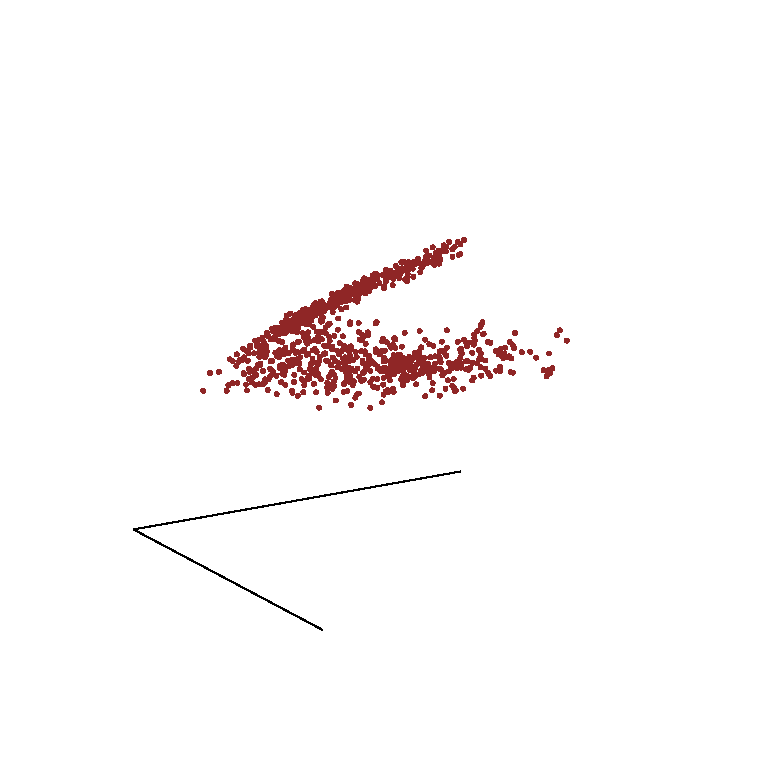
\includegraphics[width=6cm]{gnuplot/xyz.eps}};
  \end{scope}
  
  \draw [->, >=stealth, line width=1] (-5.88, -3.16) -- (-1.62, -5.43);
  \node[] at (-1.3 + \dx, -6) { $\theta_{1}$ };
  
  \draw [->, >=stealth, line width=1] (-5.88, -3.16) -- (1.58, -1.83);
  \node[] at (2.25 + \dx, -1.75) { $\theta_{2}$ };
    
  \draw [->, >=stealth, line width=1] (-5.88, -3.16) -- +(0, 7);
  \node[] at (-5.88 + \dx, 4.5) { $\theta_{3}$ };  
  
\end{tikzpicture}

\end{document}  